% Supplementary material for the PRISM-3D manuscript. Compile like main.tex.
\documentclass[11pt,a4paper]{article}
\usepackage[utf8]{inputenc}
\usepackage{mathptmx} % Times; on Overleaf you may use \usepackage[T1]{fontenc}\usepackage{lmodern} instead
\usepackage[margin=2.4cm]{geometry}
\usepackage{amsmath,amssymb,graphicx,booktabs,tabularx,xcolor}
\usepackage[round,authoryear]{natbib}
\usepackage[hidelinks]{hyperref}
\graphicspath{{figures/}}
% Each placeholder carries a key, e.g. \xyz[h1.bfree.delta]. The key names the value; it is not printed.
% python scripts/fill_results.py fills every key it can compute and lists all keys in paper_values.md.
\newcommand{\xyz}[1][]{\colorbox{yellow}{[xyz]}}
\renewcommand{\thetable}{S\arabic{table}}
\renewcommand{\thefigure}{S\arabic{figure}}
\renewcommand{\thesection}{S\arabic{section}}

\title{Supplementary Material\\ Does Explicit Monocular 3D Geometry Help AI Generated Image Detectors?}
\author{}
\date{}

\begin{document}
\maketitle

\section{Split summary and leakage report}

Table~\ref{tab:s_split} is produced from \texttt{split\_summary.csv}; the leakage checks come from \texttt{leakage\_report.json}. The run stops with an error if any check fails, so a completed run implies that all overlaps below are empty.

\begin{table}[h]
\centering
\caption{Images per set, class and generator or real source after capping and deduplication.}
\label{tab:s_split}
\small
\begin{tabular}{@{}llr@{}}
\toprule
Set & Generator or real source & Images \\
\midrule
Fit & \xyz[split.fit.sources] & \xyz[split.fit.n] \\
Validation & \xyz[split.val.sources] & \xyz[split.val.n] \\
Test A & \xyz[split.A.sources] & \xyz[split.A.n] \\
Test B & \xyz[split.B.sources] & \xyz[split.B.n] \\
Test C & \xyz[split.C.sources] & \xyz[split.C.n] \\
Test D & \xyz[split.D.sources] & \xyz[split.D.n] \\
\bottomrule
\end{tabular}
\end{table}

\begin{table}[h]
\centering
\caption{Leakage report.}
\small
\begin{tabular}{@{}lr@{}}
\toprule
Check & Value \\
\midrule
Generators shared by fit pool and tests & \xyz[leak.generator_overlap]{} (must be none) \\
Real image sources shared by fit pool and tests & \xyz[leak.real_source_overlap]{} (must be none) \\
Captions shared by fit pool and tests & \xyz[leak.prompt_overlap]{} (must be 0) \\
Captions shared by fit and validation & \xyz[leak.fitval_prompt_overlap]{} (must be 0) \\
Fit images removed as near duplicates of test images & \xyz[leak.dedup_removed] \\
Images that could not be read and were dropped & \xyz[leak.unreadable] \\
\bottomrule
\end{tabular}
\end{table}

\section{Normal convention and estimator checks}

The sign vector aligning DSINE normals with MoGe normals was \xyz[conv.sign], with a median angle of \xyz[conv.median_angle]{} degrees on 50 fit images (\texttt{geometry\_convention.json}). Missing value flag rates per class: G2 \xyz[flags.g2.real]{} (real) and \xyz[flags.g2.fake]{} (generated), G3 \xyz[flags.g3.real]{} and \xyz[flags.g3.fake], G4 \xyz[flags.g4.real]{} and \xyz[flags.g4.fake].

\section{Stacker selection}

\begin{table}[h]
\centering
\caption{Selected regularisation $C$, generator grouped cross validation AUROC, temperature and threshold for each base detector and model (from \texttt{stackers/*/*.json}).}
\small
\begin{tabular}{@{}llcccc@{}}
\toprule
Detector & Model & $C$ & CV AUROC & Temperature & Threshold (logit) \\
\midrule
B-Free & M1 to M5 & \xyz[stacker.bfree.C] & \xyz[stacker.bfree.cv_auroc] & \xyz[stacker.bfree.temperature] & \xyz[stacker.bfree.threshold] \\
CO-SPY & M1 to M5 & \xyz[stacker.cospy.C] & \xyz[stacker.cospy.cv_auroc] & \xyz[stacker.cospy.temperature] & \xyz[stacker.cospy.threshold] \\
UnivFD & M1 to M5 & \xyz[stacker.univfd.C] & \xyz[stacker.univfd.cv_auroc] & \xyz[stacker.univfd.temperature] & \xyz[stacker.univfd.threshold] \\
\bottomrule
\end{tabular}
\end{table}

\section{Additional results}

\begin{figure}[h]
\centering
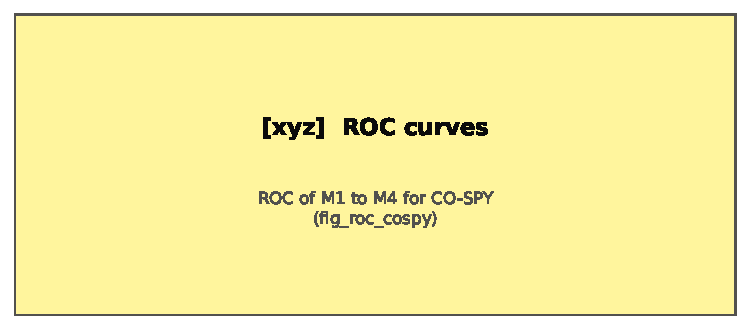
\includegraphics[width=0.45\linewidth]{fig_roc_cospy.pdf}\hfill
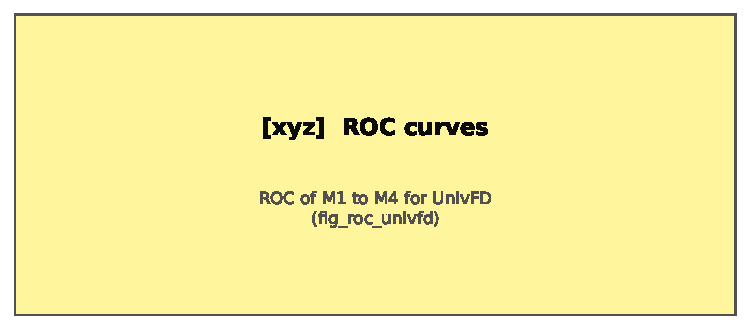
\includegraphics[width=0.45\linewidth]{fig_roc_univfd.pdf}
\caption{ROC curves of M1 to M4 for CO-SPY (left) and UnivFD (right), unseen generators.}
\end{figure}

\begin{table}[h]
\centering
\caption{Seen family generators (excluded from the headline analysis): macro AUROC of M1 and M3.}
\small
\begin{tabular}{@{}lcc@{}}
\toprule
Detector & M1 & M3 \\
\midrule
B-Free & \xyz[seen.bfree.M1] & \xyz[seen.bfree.M3] \\
CO-SPY & \xyz[seen.cospy.M1] & \xyz[seen.cospy.M3] \\
UnivFD & \xyz[seen.univfd.M1] & \xyz[seen.univfd.M3] \\
\bottomrule
\end{tabular}
\end{table}

\begin{table}[h]
\centering
\caption{Calibration (ECE, 15 bins) and accuracy on real and generated images at the fixed threshold, clean copies, pooled unseen generators.}
\small
\begin{tabular}{@{}llccc@{}}
\toprule
Detector & Model & ECE & Real accuracy & Generated accuracy \\
\midrule
B-Free & M1 / M3 & \xyz[calib.bfree.ece.M1]{} / \xyz[calib.bfree.ece.M3] & \xyz[calib.bfree.acc_real.M1]{} / \xyz[calib.bfree.acc_real.M3] & \xyz[calib.bfree.acc_fake.M1]{} / \xyz[calib.bfree.acc_fake.M3] \\
CO-SPY & M1 / M3 & \xyz[calib.cospy.ece.M1]{} / \xyz[calib.cospy.ece.M3] & \xyz[calib.cospy.acc_real.M1]{} / \xyz[calib.cospy.acc_real.M3] & \xyz[calib.cospy.acc_fake.M1]{} / \xyz[calib.cospy.acc_fake.M3] \\
UnivFD & M1 / M3 & \xyz[calib.univfd.ece.M1]{} / \xyz[calib.univfd.ece.M3] & \xyz[calib.univfd.acc_real.M1]{} / \xyz[calib.univfd.acc_real.M3] & \xyz[calib.univfd.acc_fake.M1]{} / \xyz[calib.univfd.acc_fake.M3] \\
\bottomrule
\end{tabular}
\end{table}

\section{Supplementary image level tests}

DeLong tests for M3 against M1 on pooled unseen generators gave $z$ = \xyz[delong.bfree.z]{} ($p$ = \xyz[delong.bfree.p]) for B-Free, \xyz[delong.cospy.z]{} (\xyz[delong.cospy.p]) for CO-SPY and \xyz[delong.univfd.z]{} (\xyz[delong.univfd.p]) for UnivFD (\texttt{hypotheses.json}, key \texttt{delong\_M3\_vs\_M1}). These image level tests ignore the clustering of images within generators and are reported only as a secondary analysis.

\section{Outside reference: zero shot multimodal model}

Qwen2.5-VL-7B-Instruct \citep{bai2025qwen25vl}, asked whether each image is AI generated and scored by the log probability ratio of the answers Yes and No, reached a pooled AUROC of \xyz[qwen.auroc]{} on \xyz[qwen.n]{} sampled test images. It is not part of any hypothesis test.

\bibliographystyle{plainnat}
\bibliography{references}
\end{document}
